\documentclass[a4paper,11pt]{kth-mag}
\usepackage[T1]{fontenc}
\usepackage{textcomp}
\usepackage{lmodern}
\usepackage[latin1]{}
\usepackage[swedish,english]{babel}
\usepackage{modifications}
\usepackage[numbers, longnamesfirst, sort&compress]{natbib}
\usepackage[colorlinks=true, citecolor=blue]{hyperref}
\hypersetup{linktoc=page}

%----------------------------------------------------------------
%
% Custom packages
%
%----------------------------------------------------------------
\usepackage{amsmath}
\usepackage[capitalise, nameinlink, noabbrev]{cleveref}
\usepackage{adjustbox}

\newcommand*{\skippara}{\par\vspace{\baselineskip} \noindent}


\newcolumntype{P}[1]{>{\centering\arraybackslash}p{#1}}
\newcommand\floor[1]{\lfloor#1\rfloor}
\usepackage{array}
\newcolumntype{L}[1]{>{\raggedright\let\newline\\\arraybackslash\hspace{0pt}}m{#1}}
\newcolumntype{C}[1]{>{\centering\let\newline\\\arraybackslash\hspace{0pt}}m{#1}}
\newcolumntype{R}[1]{>{\raggedleft\let\newline\\\arraybackslash\hspace{0pt}}m{#1}}
\usepackage{makecell}

\usepackage{lmodern}
\usepackage{amsmath}
\usepackage{xcolor}
\usepackage{textcomp}
\usepackage{listings}
\lstset{
    basicstyle=\footnotesize\ttfamily,
    numbers=left,
    stepnumber=1,
    columns=fullflexible,
    showstringspaces=false,
    frame=single,
    breaklines=true,
    postbreak=\mbox{\textcolor{red}{$\hookrightarrow$}\space},
}


\usepackage{pgfplotstable, booktabs}
\usepackage{color, colortbl}

%----------------------------------------------------------------
%
% Tikz
%
%----------------------------------------------------------------
\usepackage{tikz}
\usetikzlibrary{shapes.geometric,backgrounds,calc}
\tikzset{
    basic box/.style = {
        shape = rectangle,
        align = center,
        draw  = #1,
        fill  = #1!25,
        minimum width=4.4cm,
        minimum height=1cm,
        rounded corners
    },
    guest os/.style = {
        shape = rectangle,
        align = center,
        draw  = #1,
        fill  = #1!25,
        minimum width=2.15cm,
        minimum height=1cm,
        rounded corners
    },
    app guest os/.style = {
        shape = rectangle,
        align = center,
        draw  = #1,
        fill  = #1!25,
        minimum width=2.15cm,
        minimum height=1cm,
        rounded corners
    }
}

\usepackage{pgfplots}
\usepackage{graphicx}
\usepackage{lipsum}
\graphicspath{ {figures/} }

%----------------------------------------------------------------
%
% Glossary
%
%----------------------------------------------------------------
\usepackage[automake, toc, acronym, nopostdot]{glossaries}
\renewcommand*{\glstextformat}[1]{\textcolor{black}{#1}}
\makeglossaries

%%% define the acronym and use the see= option

%----------------------------------------------------------------
%
% ACRONYM
%
%----------------------------------------------------------------
\newacronym{ict}{ICT}{Information and Communication Technology}
\newacronym{lkm}{LKM}{Loadable Kernel Module}
\newacronym{nic}{NIC}{Network Interface Card}
\newacronym{vm}{VM}{Virtual Machine}
\newacronym{oci}{OCI}{Open Container Initiative}
\newacronym{rhel}{RHEL}{Red Hat Enterprise Linux}
\newacronym{cncf}{CNCF}{Cloud Native Computing Foundation}
\newacronym{cli}{CLI}{Command Line Interface}
\newacronym{mac}{MAC}{Media Accecs Protocol}
\newacronym{ipv4}{IPv4}{Internet Protocol version 4}
\newacronym{ipv6}{IPv6}{Internet Protocol version 6}
\newacronym{vlan}{VLAN}{Virtual Local Area Network}
\newacronym{arp}{ARP}{Address Resolution Protocol}
\newacronym{http}{HTTP}{Hypertext Transfer Protocol}
\newacronym{udp}{UDP}{User Datagram Protocol}
\newacronym{tcp}{TCP}{Transport Control Protocol}
\newacronym{sctp}{SCTP}{Stream Control Transmission Protocol}
\newacronym{vxlan}{VXLAN}{Virtual Extensible LAN}
\newacronym{isp}{ISP}{Internet Service Provider}
\newacronym{gui}{GUI}{Graphical User Interface}
\newacronym{ssh}{SSH}{Secure Shell}
\newacronym{nat}{NAT}{Network Address Translation}
\newacronym{dpdk}{DPDK}{Data Plane Development Kit}
\newacronym{api}{API}{Application Programming Interface}
\newacronym{lxc}{LXC}{Linux Containers}
\newacronym{mbps}{Mbps}{Megabit per second}
\newacronym{gbps}{Gbps}{Gigabit per second}
\newacronym{cpu}{CPU}{Central Processing Unit}
\newacronym{devops}{DevOps}{Development and Systems Operation}
\newacronym{os}{OS}{Operating System}
\newacronym{it}{IT}{Information Technology}
\newacronym{app}{APP}{Application software}


\title{An Evaluation of Software-Based \\Traffic Generators using Docker}
\subtitle{}
\foreigntitle{En Utv\"ardering utav Mjukvarubaserade Trafikgeneratorer med Docker}
\author{Sai Man Wong}
\date{}
\blurb{Master's Thesis in Computer Science at \\
School of Computer Science and Communication, KTH
\\~\\
Supervisor: Alexander Kozlov\\
Examiner: Joakim Gustafson}
\trita{}
\begin{document}
\frontmatter
\pagestyle{empty}
\removepagenumbers
\maketitle
%----------------------------------------------------------------
%
% ABSTRACT
%
%----------------------------------------------------------------
\selectlanguage{english}
\begin{abstract}
    The \gls{ict} industry and network researchers use traffic generator tools to a large extent to test their systems.
    The industry uses reliable and rigid hardware-based platform tools for high-performance network testing.
    The research community commonly uses software-based tools in, for example, experiments because of economic and flexibility aspects.
    As a result, it is possible to run these tools on different systems and hardware.
    In this thesis, we examine the software traffic generators Iperf, Mausezahn, Ostinato in a closed loop physical and virtual environment,
    that is, to evaluate the applicability of the tools and find sources of inaccuracy for a given traffic profile.
    For each network tool, we measure the throughput from 64- to 4096-byte in packet sizes.
    Also, we encapsulate each tool with container technology using Docker to reach a more reproducible and portable research.
    Our results show that the \acrshort{cpu} primarily limits the throughput for small packet sizes, and saturates the 1000 \acrshort{mbps} link for larger packet sizes.
    Finally, we suggest using these tools for simpler and automated network tests.
\end{abstract}
\clearpage
\begin{foreignabstract}{swedish}
    IT-branschen och n\"{a}tverksforskare anv\"{a}nder sig av trafikgeneratorer till stor del f\"{o}r att testa sina system.
    Industrin anv\"{a}nder sig av stabila och p\r{a}litliga h\r{a}rdvaruplattformar f\"{o}r h\"{o}gpresterande n\"{a}tverkstester.
    Forskare brukar anv\"{a}nda mjukvarubaserade verktyg i till exempel experiment p\r{a} grund av ekonomiska och flexibilitet sk\"{a}l.
    Det \"{a}r d\"{a}rf\"{o}r m\"{o}jligt att anv\"{a}nda dessa verktyg p\r{a} olika system och h\r{a}rdvaror.
    I denna avhandling unders\"{o}ker vi mjukvaru-trafikgeneratorerna Iperf, Mausezahn, Ostinato i en isolerad fysisk och virtuell milj\"{o}, det vill s\"{a}ga f\"{o}r att utv\"{a}rdera anv\"{a}ndbarheten av verktygen och hitta felk\"{a}llor f\"{o}r en given trafikprofil.
    F\"{o}r varje n\"{a}tverksverktyg m\"{a}ter vi genomstr\"{o}mningen fr\r{a}n 64 till 4096 byte i paketstorlekar.
    Dessutom paketerar vi varje verktyg med molnteknologin Docker f\"{o}r att n\r{a} ett mer reproducerbart och portabelt arbete.
    V\r{a}ra resultat visar att processorn begr\"{a}nsar genomstr\"{o}mningen f\"{o}r sm\r{a} paketstorlekar och saturerar 1000 Mbps-l\"{a}nken f\"{o}r st\"{o}rre paketstorlekar.
    Slutligen f\"{o}resl\r{a}r vi att man kan anv\"{a}nda dessa verktyg f\"{o}r enklare och automatiserade n\"{a}tverkstester.
\end{foreignabstract}


%----------------------------------------------------------------
%
% Acknowledgements
%
%----------------------------------------------------------------
% \chapter*{Acknowledgements}
% \lipsum[1]
% \clearpage
% \null\clearpage
%----------------------------------------------------------------
%
% TABLE OF CONTENTS
%
%----------------------------------------------------------------
\clearpage
\tableofcontents*
\listoffigures
\clearpage
\listoftables
\printglossary[nonumberlist, type=\acronymtype]
\clearpage
\mainmatter

\pagestyle{newchap}
%----------------------------------------------------------------
%
% CHAPTER
%
%----------------------------------------------------------------
\chapter{Introduction}\label{introduction}

\acrfull{ict} companies, for example, cloud service providers and mobile network operators provide reliable network products, services or solutions to handle network traffic on a large scale.
These companies rely on proprietary and hardware-based network testing tools to test their products before deployment.
That is, to generate realistic network traffic, which is then injected into a server to verify its behavior.
Because of high demand to send and receive information with high speed and low latency, it is essential to test the \gls{ict} solutions thoroughly.

%----------------------------------------------------------------
%
% Problem
%
%----------------------------------------------------------------
\section{Problem Statement}

In contrast to \gls{ict} enterprises, the network research community develops and uses open-source and software-based network testing tools.
Thus, researchers use software-based network testing tools \cite{DITGDist48:online, Packetge32:online, ToolsThe22:online} in experiments because of its flexibility and for economic reasons \cite{botta2010you, molnar2013validate}.
However, the generated network traffic from these tools is not as reliable as the one from the hardware-based platform, because of the underlying hardware and software, such as \gls{nic} and \gls{os}.
Use of the software-based tools without an awareness of these variables, can produce inaccurate results between the generated and requested network traffic.

\skippara This paper examines the software-based network traffic generators Iperf, Mausezahn, and Ostinato.
The purpose is to test the chosen tools concerning accuracy for different network profile, and the efficiency with lightweight hardware and software typical for academic environments.
Distinctively to other similar studies, this project uses the container technology Docker to encapsulate the tools for automated tests and to achieve a higher degree of a reproducibility \cite{piccolo2016tools, boettiger2015introduction, Chamberlain2014}.

%----------------------------------------------------------------
%
% Limitation
%
%----------------------------------------------------------------
\section{Limitation}
Our study only investigates software-based traffic generators that primarily operate in user space and uses the Linux networking stack.

%----------------------------------------------------------------
%
% Sustainability, Ethics, and Societal Aspects
%
%----------------------------------------------------------------
\section{Sustainability, Ethics, and Societal Aspects}
In modern life, the Internet is an integral part of the human environment, where stability, security, and efficiency are the essential aspects.
This project has no direct and significant impact on sustainability in general.
Except, the power consumption of laptops with the purpose to gather data.


\skippara From an ethical standpoint, we documented our steps throughout our thesis, provided the code in the appendices, and in a public repository \url{https://github.com/saimanwong/mastersthesis}.
That is, to contribute to reproducible research and transparency.
Hence, other people are encouraged to try to replicate and achieve similar results.
However, and most likely, the results can vary because of the underlying hardware and software.

\skippara Since this project only uses open source software, it is just morally right to make everything public.
Also, the network tools used in this project are purposely for private and controlled labs or virtual environments.
Thus, it is inadvisable to use these tools on public networks.

\chapter{Background}\label{background}
%----------------------------------------------------------------
%
% Traffic Generator
%
%----------------------------------------------------------------
\section{Traffic Generator}\label{sec:tg}
The more the \gls{it} infrastructures and networks grow, the higher the demand there is to test and validate its behavior as more devices connect.
The network providers and researchers use traffic generator tools to a large extent for experiments, performance testing, verification and validation~\cite{botta2010you, molnar2013validate}.
As pointed out in the recent studies the network testing tools are either software- or hardware-based platforms~\cite{turull2016pktgen, emmerich2015moongen, antichi2014osnt, ghobadi2012caliper}.

\subsection{Why Software-Based Traffic Generator}
The network research community commonly uses or develops, open-source and software-based networking tools.
In contrast, network equipment and solution providers often use proprietary and hardware-based ones, for example, Spirent~\cite{Networkd93:online} and Ixia~\cite{IxiaMake81:online}.
These are proprietary and specialized software and hardware for network testing.
Flexibility, accuracy, and cost are the factors for this general division between hardware- and software-based platforms.
That is, 1) software-based networking tools are more flexible and cheaper than the hardware-based platform, on the other hand, 2) hardware-based tools generate more accurate and realistic network traffic than software-based tools at higher rates.

\skippara \citet*{botta2010you} identified that the flexibility of software-based network tools narrows down to three points.
First, the ease to deploy these tools in a distributed fashion.
Second, the freedom to make changes to fit a specific research purpose.
Third, it can run on top of a variety of \glspl{os} and its networking stack.
However, a hardware-based platform is more rigor and stable for network testing, because of its specialization.

\skippara The traffic's accuracy comes down to how well a network provider can fulfill the customer's requirements, for example, a mobile operator or an \gls{isp}.
These profiles are often rigor and detailed data sheets that describe, for example, a specified speed or correctness within an error interval.
Software-based tools often do not meet these requirements.
That is, without knowledge of underlying hardware and software, there is a high chance to produce inaccurate results.
Thus, \citet*{botta2010you} examined four software traffic generators and tried to raise awareness within the network research community to assess traffic generators critically.

\subsection{Metrics and Types}\label{metrictype}
There is a vast amount of software-based traffic generators with different purposes, for example, \cite{DITGDist48:online, Packetge32:online, ToolsThe22:online} are three lists of traffic generators to only mention a few.
Therefore, \citet{botta2010you, molnar2013validate} have attempted to categorize most frequently used traffic generators in the papers ``Do you trust your software-based traffic generator'' and ``How to validate traffic generators?'' respectively.
Both found that the most frequently used traffic generators in literature are packet-level and maximum throughput traffic generators, which we marked with an asterisk in \cref{types}.
Moreover, conventional metrics are byte throughput, packet size, and inter-departure/packet time distribution.

\begin{table}[ht!]
    \scriptsize
    \caption{Summary of Traffic Generators Types \cite{botta2010you, molnar2013validate}}
    \label{types}
    \begin{adjustbox}{center}
        \renewcommand*\arraystretch{1.5}\begin{tabular}{| L{5cm} | L{8cm} |}
            \hline
            \textbf{Replay Engines} & Replay network traffic back to specified \gls{nic} from a file which contains prerecorded traffic, usually a pcap-file.
            \\ \hline
            \textbf{(*) Maximum Throughput Generators} & Generate maximum of network traffic with the purpose to test overall network performance, for example, over a link.
            \\ \hline
            \textbf{Model-Based Generators} & Generate network traffic based on stochastic models.
            \\ \hline
            \textbf{High-Level and Auto-Configurable Generators} & Generate traffic from realistic network models and change the parameters accordingly.
            \\ \hline
            \textbf{Special Scenario Generators} & Generate network traffic with a specific characteristic, for example, video streaming traffic.
            \\ \hline \hline
            \textbf{Application-level Traffic generators} & Generate network traffic of network applications, for example, the traffic behavior between servers and clients.
            \\ \hline
            \textbf{Flow-Level Traffic generators} & Generate packets in a particular order that resembles a particular characteristic from source to destination, for example, Internet traffic.
            \\ \hline
            \textbf{(*) Packet-Level Traffic Generators} & Generate and craft packets, usually, from layer 2 and up to 7.
            \\ \hline
        \end{tabular}
    \end{adjustbox}
\end{table}


\skippara On a surface level, it is also possible to divide software-based traffic generators into three general categories:
network software tools that run in user space/kernel space or circumvent the default kernel via framework to send and capture traffic.

\clearpage
\subsubsection{User Space}
Userspace traffic generators often use the library libpcap for Unix-like systems or WinPcap for Windows system \cite{Programm92:online}.
That is, a library to access the default network stack that primarily uses system calls, such as socket \acrshort{api}, to capture and inject packets.
For instance, the network tools like Iperf \cite{iPerfThe63:online}, Mausezahn \cite{netsniff7:online}, Ostinato \cite{Ostinato63:online} and Tcpdump \cite{TCPDUMPL66:online}.

\subsubsection{Kernel Space}
These tools are primarily developed as a \gls{lkm} and run close to the physical hardware, such as the \gls{nic}.
Thus, they introduce little processing overhead compared to userspace tools.
There are fewer context switches between user and kernel space, and as a consequence, such tools generate synthetic network traffic more efficient, for example, Brute \cite{bonelli2005brute} and Pktgen \cite{turull2016pktgen}.

\subsubsection{External Framework}
The Linux network stack is complex and designed for general purpose.
However, it is not explicitly designed for packet processing at higher rates, especially for small packets.
\citet{gallenmuller2015comparison} examined the software frameworks to circumvent the standard Linux network stack, that is, the frameworks netmap \cite{infoietu32:online}, \acrshort{dpdk} \cite{DPDK35:online} and PF\_RING \cite{PFRINGn1:online}.
In comparison to the Linux network stack, the authors concluded: ``The performance increase comes from processing in batches, preallocated buffers, and avoiding costly interrupts''.
For example, MoonGen \cite{emmericp44:online} and TRex \cite{TRex62:online} are two traffic generators built on DPDK.

\subsection{Known Bottlenecks}
For packet processing application that uses the Linux network stack, the common bottlenecks are the processor, memory, software design and cache size \cite{raumer2015performance, emmerich2015assessing, braun2010comparing, gallenmuller2015comparison}.
Most of the applications can reach 1 Gbps on the default network stack.
Above this rate, for example, at the rate of 10 \acrshort{gbps}, noticeable limits appear.

\skippara Firstly, the \acrshort{cpu} limits the tool to craft more complex packets.
For example, the traffic generator uses $x$ cycles to process a single packet, which may lead the \acrshort{cpu} to go on full workload for a more substantial number of packets to process.
Secondly, \texttt{sk\_buff}, a data structure that stores information about a packet, is large and complex \cite{networki54:online}.
It becomes costly to allocate and deallocate memory for the packets at high rates.
Thirdly, software design comes down to, for example, the packet queue gets stuck in a spinlock.
As a result, \acrshort{cpu} cycles go to waste due to the wait.
Finally, the \acrshort{cpu} cache size influences cache hits, miss and \acrshort{cpu} cycles.
For example, with a larger \acrshort{cpu} cache, the chances are higher to get cache hits and minimize \acrshort{cpu} idle for packet processing.


%----------------------------------------------------------------
%
% Virtualization
%
%----------------------------------------------------------------
\section{Virtualization}

MIT and IBM introduced the concept of virtualization in the 1960s~\cite{daniels2009server}.
Now, in the 21st century, cloud computing has become one of the mainstream technology, and virtualization is the core of it~\cite{srinivasan2014cloud}.
That is a technology to partly or entirely separate software services from the physical hardware.

\skippara Virtualization technology enables multiple and isolated instances of a guest \gls{os} to share the same hardware resources~\cite{cherkaoui2014virtualization}.
An instance of a guest \gls{os} is therefore often called a \gls{vm} or virtual server.
Thus, today it is common that more than ten instances run on a single physical server, but each of these operates as its virtual machine.
For example, a physical server runs Ubuntu as the host \gls{os}.
On top of the hardware and Ubuntu, virtualization makes it then possible to run various guest \gls{os}s upon it seamlessly, such as Windows and other Unix-like \gls{os}s.


\skippara Virtualization is commonly related to servers and categorized into three types.
The server virtualization types are 1) full virtualization, 2) paravirtualization and 3) \gls{os} virtualization~\cite{bauer2012reliability}.
The two former types use a hypervisor, and the latter does not, see~\cref{fig:virtualization}.
A hypervisor is a layer between the underlying hardware and virtual machines.
Its purpose is to manage and allocate hardware resources to the virtual machines.
There are two types of hypervisors, type 1 and type 2.
\skippara In short, type 1 hypervisor integrates a layer in the hardware system as firmware.
This type is also called a bare metal hypervisor because it is directly on top of the hardware.
It provides high performance, but also high complexity as it requires modification of the \gls{os}.
Finally, a type 2 hypervisor runs, as software, on the host \gls{os} to achieve virtualization.
This approach is flexible but introduces high overhead compared to type.
Both of these types can run multiple and entire \gls{os}s as virtual machines.
In contrast, \gls{os} virtualization is a lighter version of virtualization, does not run entire \gls{os}s and require no hypervisor.

\begin{figure}[h!]
    \centering
    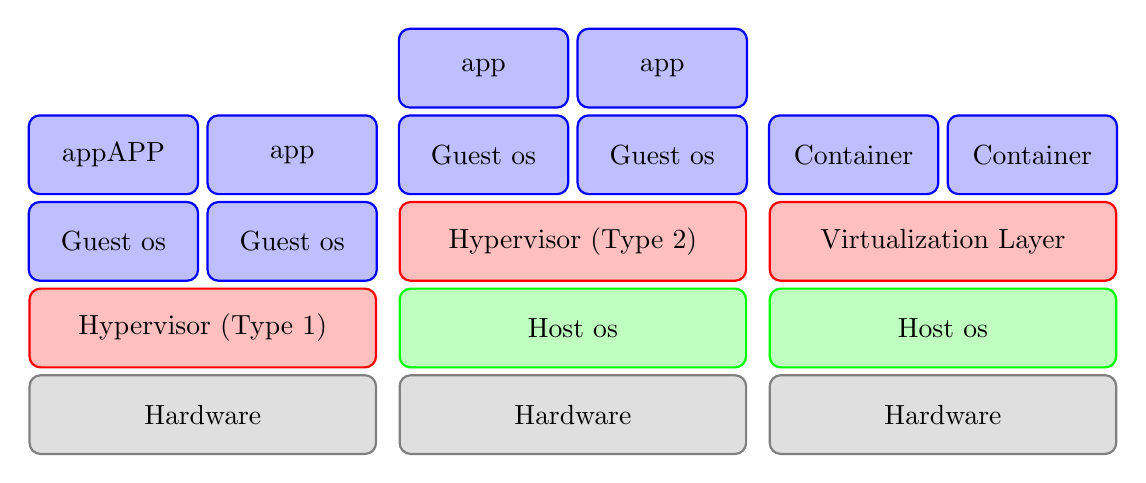
\begin{tikzpicture}[node distance = 1.2cm, thick, nodes = {align = center}, >=latex]
      \node at (0,0) [basic box = gray] {Hardware};
      \node at (0,1.1) [basic box = red] {Hypervisor (Type 1)};
      \node at (-1.135, 2*1.1) [guest os = blue] {Guest \gls{os}};
      \node at (1.135, 2*1.1) [guest os = blue] {Guest \gls{os}};
      \node at (-1.135, 3*1.1) [guest os = blue] {\glsdisp{app}{APP}};
      \node at (+1.135, 3*1.1) [guest os = blue] {\gls{app}};

      \node at (4.7, 0) [basic box = gray] {Hardware};
      \node at (4.7, 1.1) [basic box = green] {Host \gls{os}};
      \node at (4.7,2*1.1) [basic box = red] {Hypervisor (Type 2)};
      \node at (4.7-1.135, 3*1.1) [guest os = blue] {Guest \gls{os}};
      \node at (4.7+1.135, 3*1.1) [guest os = blue] {Guest \gls{os}};
      \node at (4.7-1.135, 4*1.1) [guest os = blue] {\gls{app}};
      \node at (4.7+1.135, 4*1.1) [guest os = blue] {\gls{app}};

      \node at (2*4.7, 0) [basic box = gray] {Hardware};
      \node at (2*4.7, 1.1) [basic box = green] {Host \gls{os}};
      \node at (2*4.7, 2*1.1) [basic box = red] {Virtualization Layer};
      \node at (9.4-1.135, 3*1.1) [guest os = blue] {Container};
      \node at (9.4+1.135, 3*1.1) [guest os = blue] {Container};
    \end{tikzpicture}
  \caption{Hypervisor-Based (Type 1 and 2) and Container-Based Virtualization}
  \label{fig:virtualization}
\end{figure}


\subsection{Operating System Virtualization (Containers)}\label{background:osvirtual}

An operating system virtualization approach enables isolation of instances in user space without a hypervisor.
Instead, this type uses system calls and other system \gls{api} primarily to access the kernel and its hardware resources~\cite{bauer2012reliability}.
An instance of such is called a container; hence, this approach is also often referred to as container-based virtualization or container technology.

\hfill\break
\hfill\break
\hfill\break

\skippara Containers use the same resources as the host \gls{os} kernel to achieve isolated virtual environments, that is, in contrast to virtual machines that use a hypervisor.
This approach uses kernel features typically to run separated containers~\cite{xavier2013performance, namespac0:online}.
Thus, containers must support the host \gls{os} and its kernel to run, for example, a Linux distribution, such as CentOS, Ubuntu or \gls{rhel}.

\skippara \citet*{joy2015performance} identified four reasons container technology has been and is gaining popularity among developers, \gls{it} architects and operation persons.

\skippara \textbf{``Portable Deployments''} allows encapsulation of applications, and can then a developer can deploy these on many different systems.
\skippara \textbf{``Fast application delivery''} facilitates the product pipeline because the applications never leave the containers throughout the development, testing, and deployment stages. Also, a large part of this process, if not entire, can be automated with containers.
\skippara \textbf{``Scale and deploy with ease''} allow straightforward transfer of containers between the desktop, dedicated server or cloud environments. Also, it is easy to run and stop hundreds of containers.
\skippara \textbf{``Higher workloads with greater density''} allow more guest virtual environments (containers) to run on the host, that is, does not run entire \gls{os} as a virtual machine with a hypervisor, and thus, container technology introduces little to no overhead.

\skippara In parallel with cloud computing, \gls{os} virtualization or container technology evolved into open-source projects that are part of the Linux Foundation.

\clearpage
\subsection{Docker}\label{background:docker}
The concept of containers grew incrementally from 1979 till at the time of writing \cite{TheEvolu99:online, Momentsi23:online, ABriefHi14:online, TheHisto4:online, AboutOp82:online}.
It began with unsecured and partly isolated virtual environments.
In 2015, leaders within the container industry started the project \gls{oci} as part of the Linux Foundation to establish a standard for containers, that is, the \gls{oci} specification~\cite{AboutOp82:online, Projects37:online}.
Among these industry leaders, Docker is one of the driving forces behind this project.
\cref{fig:trend} shows the popularity of Docker in recent years compared to other container technology approaches.


\skippara Docker is an open-source software platform built on Moby~\cite{mobymoby68:online, WhatisDo49:online}.
It is a platform that enables development, provisioning, and deployment of software insecure and isolated containers.
Docker's  first iteration of the platform built upon \gls{lxc} to manage containers.
However, several iterations later, \gls{lxc} was replaced with their library called libcontainer \cite{dockerli21:online}.
Finally, they donated libcontainer as runc to \gls{oci}, and containerd to \gls{cncf}, both are Linux Foundation projects~\cite{opencont67:online, containe72:online}.

\begin{figure}[h!]
    \centering
    \includegraphics[width=13cm]{figure/trend}
    \caption{Google Trends of Container Technology (May 28, 2017)}
    \label{fig:trend}
\end{figure}

\skippara \cref{fig:arch} shows a high-level view of Docker's architecture
That is, the user uses (1) \gls{cli}-commands to interact with (2) Docker engine to manage Docker images, containers, network configurations, orchestration and more.
(3) containerd spins up container based on \gls{oci} container industry standard, such as (4) runc.
However, the fundamentals of container lie primarily around the Linux kernel features cgroups and namespaces.
In other words, cgroups ``limits how much you can use'' and namespaces ``limits what you can see (and therefore use)'' \cite{Anatomyo69:online}.

\begin{figure}[h!]
    \centering
    \includegraphics[width=11cm]{figure/dockerarchblog}
    \caption{Overview of Docker Architecture~\cite{Docker1199:online}}
    \label{fig:arch}
\end{figure}

\skippara Docker is feature rich in different ways to manage containers.
The following simplifies and describes a few Docker fundamentals.
That is, there are more advanced features that require specific \gls{cli}-flags to achieve a particular purpose.

\subsubsection{Docker Image}
Docker image is like a template, for example, a class in object-oriented programming.
An image contains different layers of the file system, for example, layer 1) Ubuntu base image and layer 2) updated packages.
Then, on top of all other layers, there is finally only a read-only file system layer.
It is possible to inspect the different layers of a Docker image with:
\begin{lstlisting}[numbers=none, frame=single]
  $ docker history <IMAGE_NAME:TAG>
\end{lstlisting}

\skippara There are two ways to create a Docker image. Either use already running container:
\begin{lstlisting}[numbers=none, frame=single]
  $ docker commit <RUNNING_CONTAINER> <IMAGE_NAME:TAG>
\end{lstlisting}

\skippara alternatively, build an image from a human-readable and portable file called Dockerfile:
\begin{lstlisting}[numbers=none, frame=single]
  $ docker build -t <IMAGE_NAME:TAG> <PATH_TO_DOCKERFILE_DIR>
\end{lstlisting}

\clearpage
\subsubsection{Docker Container}
Docker container is a running instance of an image, for example, an object in object-oriented programming.
Thus, once a container is running, it can then use the same hardware resources as the host kernel, such as file system, memory, \acrshort{cpu}, network, user and more.
For example:
\begin{lstlisting}[numbers=none, frame=single]
  $ docker run <IMAGE_NAME:TAG>
\end{lstlisting}

\skippara In our experiments, we followed the container technology standards to package the software in light-weight and portable containers.
It enabled us to move the software between environments with the dependencies intact more easily.
Also, the method to containerize the software facilitated the automation process of the tests.

\chapter{Related Work}\label{relatedwork}

In past research on traffic generators \cite{botta2010you, turull2016pktgen, kolahi2011performance, srivastava2014evaluation, srivastava2014comparative}, were conducted experiments in a closed-loop environment between two hosts connected via a link.
All these experiments included throughput test on traffic generators, in either packet per second or bit rate.
As mentioned in \cref{metrictype}, the network research community frequently uses the metrics byte throughput and packet size.
We try to focus on the following metrics in our project.
In \cite{kolahi2011performance, srivastava2014evaluation, srivastava2014comparative}, the authors conducted similar throughput experiments with userspace tools, and we used their method as inspiration for this project.

\skippara In \cite{kolahi2011performance}, the authors generated \acrshort{tcp} traffic over a 100 \acrshort{mbps} link, packet sizes ranging from 128 to 1408 bytes, and used the tools Iperf, Netperf, D-ITG and IP Traffic.
The authors in \cite{srivastava2014evaluation, srivastava2014comparative} generated both \acrshort{tcp} and \acrshort{udp} traffic over 10 and 40 \acrshort{gbps} links respectively, packet sizes between 64 and 8950 bytes, and with Iperf, PackETH, Ostinato, and D-ITG.
The results are similar in all these experiments, in the sense that the throughput increases for larger packet sizes because small packet sizes introduce higher overhead and cause lower performance.
\cref{table:experimentsummary} summarizes the highest throughput from these experiments.

\begin{table}[ht!]
    \scriptsize
    \caption{Maximal Throughput Summary of \cite{kolahi2011performance, srivastava2014evaluation, srivastava2014comparative}}
    \label{table:experimentsummary}
    \begin{adjustbox}{center}
        \renewcommand*\arraystretch{1.5}\begin{tabular}{| L{1.6cm} | L{1.7cm} | L{1.7cm} | L{1.7cm} || L{1.7cm} | L{1.7cm} |}

            \hline
            \textbf{Tools} & \textbf{\cite{kolahi2011performance} \acrshort{tcp}} & \textbf{\cite{srivastava2014evaluation} \acrshort{tcp}} & \textbf{\cite{srivastava2014comparative} \acrshort{tcp}} & \textbf{\cite{srivastava2014evaluation} \acrshort{udp}} & \textbf{\cite{srivastava2014comparative} \acrshort{udp}}
            \\ \hline
            D-ITG & 83.8 \acrshort{mbps} & 6520 \acrshort{mbps} & 16.2 \acrshort{gbps} & 7900 \acrshort{mbps} & 26.7 \acrshort{gbps}
            \\ \hline
            Iperf & \textbf{93.1 \acrshort{mbps}} & 5400 \acrshort{mbps} & - & 1.05 \acrshort{mbps} & -
            \\ \hline
            Ostinato & - & \textbf{9000 \acrshort{mbps}} & 38.8 \acrshort{gbps} & 9890 \acrshort{mbps} & 36.9 \acrshort{gbps}
            \\ \hline
            PackETH & - & 7810 \acrshort{mbps} & \textbf{39.8 \acrshort{gbps}} & \textbf{9980 \acrshort{mbps}} & \textbf{39.8 \acrshort{gbps}}
            \\ \hline
            IP Traffic & 76.7 \acrshort{mbps} & - & - & - & -
            \\ \hline
            Netperf & 89.9 \acrshort{mbps} & - & - & - & -
            \\ \hline \hline
            Iperf multithread & - & 9540 \acrshort{mbps} & - & 12.6 \acrshort{mbps} & -
            \\ \hline
            D-ITG multithread & - & 9820 \acrshort{mbps} & 39.9 \acrshort{gbps} & 8450 \acrshort{mbps} & 39.8 \acrshort{gbps}
            \\ \hline
        \end{tabular}
    \end{adjustbox}
\end{table}


\skippara In latterly mentioned experiments, we encountered two observations that could make it harder for us to reproduce.
First, they used network tools with either an architecture to both send and capture traffic or only send.
Therefore, it is unclear what method they used to monitor the traffic.
Second, we could not find which version of the network tools they used.
To avoid ambiguity and to make our project more reproducible, we packaged the tools into different Docker containers, which makes them easy to deploy on various of systems.
In our study, we try to evaluate the limits of userspace traffic generators used in Docker container environment.
Finally, \cite{felter2015updated, chung2016using} showed that Docker containers are feasible for data-intensive applications, and reach close to native \acrshort{cpu} and memory performance, because these share the same resources as the host \acrshort{os}.


\skippara Alternatively to our approach and as examined in \cref{metrictype}, other network testing tools operate in the kernel space, or use external libraries to circumvent the host kernel and directly access commodity \acrshort{nic} to achieve faster packet processing.
In \cite{turull2016pktgen}, the authors developed the kernel module and traffic generator called Pktgen.
They ran throughput, latency and packet delay variation experiments between two machines to compare their tool to the userspace tools Iperf and Netperf; as well as Pktgen-\acrshort{dpdk} and Netmap, which use an external framework to process packets, such as \acrshort{dpdk}.
In the maximal throughput experiment for \acrshort{udp} traffic at 64 bytes packet size, former tools achieved between 150 and 350 \acrshort{mbps}, Pktgen generated a throughput of 4200 \acrshort{mbps}, and both the latter types saturated the link at 7600 \acrshort{mbps}.
MoonGen is another high-speed and \acrshort{dpdk}-based traffic generator.
The creators of MoonGen generated \acrshort{udp} traffic at minimal packet size and also saturated a 10 \acrshort{gbps} link at a lower clock frequency than Pktgen-\acrshort{dpdk} \cite{emmerich2015moongen}.
We compare and summarize our method to other related studies in \cref{tab:comparesummary}.


\skippara All the related studies used the similar experimental methodology to examine software generators.
That is, to conduct tests in an isolated environment of two machines to avoid external influences.
Naturally, traffic generators built closer to the hardware perform significantly better than userspace tools.
However, the hardware and software become more adaptable and cheaper; we decided to further examine the performance of userspace tools and their use cases.
Also, to enable \acrshort{devops}\footnote{\gls{devops} -- It is a software development philosophy, which a large number of automation and monitoring tools arose.
Of which, Docker is one of the leading tools on the market.
The author in \cite{boettiger2015introduction} describes the \acrshort{devops} methodology as: ``The approach is characterized by scripting, rather than documenting, a description of
the necessary dependencies for software to run, usually
from the Operating System (\acrshort{os}) on up.''
} practices with container technology to more efficiently automate tests in a standardized manner.

\clearpage

\begin{table}
\caption{Comparison and Summary Table of Related Work}
\label{tab:comparesummary}
\centering
{\tiny\begin{tabular}{|>{\centering\arraybackslash}m{9mm}|m{30mm}|m{35mm}|m{55mm}|}

\hline
\multicolumn{1}{|>{\centering\arraybackslash}m{9mm}|}{}
& \multicolumn{1}{>{\centering\arraybackslash}m{30mm}|}{\textbf{Traffic Generator}}
& \multicolumn{1}{>{\centering\arraybackslash}m{35mm}|}{\shortstack[c]{\\ \textbf{Metrics} \\ frequently used \\ in literature indentified \\ by \cite{molnar2013validate}}}
& \multicolumn{1}{>{\centering\arraybackslash}m{55mm}|}{\textbf{Lab Environment}}\\
        \hline
        2017 Our Work
        & \shortstack[l]{\\ User Space \\ $-$ Iperf \\ $-$ Mausezahn \\ $-$ Ostinato}
        & \shortstack[l]{\\ $-$ Byte Throughput \\ $-$ Packet Size \\ \hspace{2.5mm} Distribution}
        & \shortstack[l]{\\ Physical Lab \\ $-$  Intel Core i5-2540M \acrshort{cpu} \\ $-$ 8 GB Memory \\ $-$ 1000 \acrshort{mbps} \acrshort{nic} \\ $-$ Ubuntu Server 16.04.2 \\ $-$ Linux kernel version 4.4.0 \\ $-$ Docker version 17.05.0-ce \\ \ \\ Virtual Lab \\ \quad Host \\ \qquad $-$ Intel Core i5-5257U \acrshort{cpu} \\ \qquad $-$ 8 GB Memory \\ \qquad $-$ macOS 10.12.5 \\ \qquad $-$ Oracle VM VirtualBox 5.1.22 \\ \quad Guest \\ \qquad $-$ 1 CPU \\ \qquad $-$ 2 GB Memory \\ \qquad $-$ Ubuntu server 16.04.2 \\ \qquad $-$ Linux kernel version 4.4.0 \\ \qquad $-$ Docker version 17.05.0-ce}
        \\
        \hline
        \hline
        2016 \cite{turull2016pktgen}
        & \shortstack[l]{\\ User Space \\ $-$ Netperf \\ $-$ Iperf \\ \ \\ Kernel Space \\ $-$ Pktgen \\ \ \\ External Framework \\ $-$ Netmap  \\ $-$ Pktgen-\acrshort{dpdk}}
        & \shortstack[l]{\\ $-$ Byte Throughput \\ $-$ Packet Size \\ \hspace{2.5mm} Distribution \\ $-$ Inter Packet Time \\ \hspace{2.5mm} Distribution}
        & \shortstack[l]{\\ Physical Lab \\ $-$ Intel Xeon \acrshort{cpu} \\ $-$ 3 GB Memory \\ $-$ 10 \acrshort{gbps} \acrshort{nic} \\ $-$ Ubuntu 13.10 \\ $-$ Linux kernel version 3.18.0}
        \\
        \hline
        \hline
        2015 \cite{emmerich2015moongen}
        & \shortstack[l]{\\ External Framework \\ $-$ MoonGen  \\ $-$ Pktgen-\acrshort{dpdk}}
        & \shortstack[l]{\\ $-$ Byte Throughput \\ $-$ Packet Size \\ \hspace{2.5mm} Distribution \\ $-$ Inter Packet Time \\ \hspace{2.5mm} Distribution}
        & \shortstack[l]{\\ Physical/Virtual Lab \\ $-$ Intel Xeon \acrshort{cpu} \\ $-$ 1/10/40 \acrshort{gbps} \acrshort{nic} \\ $-$ Debian \\ $-$ Linux kernel version 3.7 \\ $-$ Open vSwitch 2.0.0}
        \\
        \hline
        \hline
        2014 \cite{srivastava2014comparative}
        & \shortstack[l]{\\ User Space \\ $-$ D-ITG  \\ $-$ Ostinato \\ $-$ PackETH}
        & \shortstack[l]{\\ $-$ Byte Throughput \\ $-$ Packet Size \\ \hspace{2.5mm} Distribution}
        & \shortstack[l]{\\ Physical Lab \\ $-$ Intel Xeon \acrshort{cpu} \\ $-$ 40 \acrshort{gbps} \acrshort{nic} \\ $-$ CentOS 6.5 \\ $-$ Linux kernel version 2.6.32}
        \\
        \hline
        \hline
        2014 \cite{srivastava2014evaluation}
        & \shortstack[l]{\\ User Space \\ $-$ D-ITG  \\ $-$ Iperf \\ $-$ Ostinato \\ $-$ PackETH}
        & \shortstack[l]{\\ $-$ Byte Throughput \\ $-$ Packet Size \\ \hspace{2.5mm} Distribution}
        & \shortstack[l]{\\ Physical Lab \\ $-$ Intel Xeon \acrshort{cpu} \\ $-$ 64 GB Memory \\ $-$ 10 \acrshort{gbps} \acrshort{nic} \\ $-$ CentOS 6.2 \\ $-$ Linux kernel version 2.6.32}
        \\
        \hline
        \hline
        2011 \cite{kolahi2011performance}
        & \shortstack[l]{\\ User Space \\ $-$ D-ITG  \\ $-$ IP-Traffic \\ $-$ Iperf \\ $-$ Netperf}
        & \shortstack[l]{\\ $-$ Byte Throughput \\ $-$ Packet Size \\ \hspace{2.5mm} Distribution}
        & \shortstack[l]{\\ Physical Lab \\ $-$ Intel Pentium 4 \acrshort{cpu} \\ $-$ 1 GB Memory \\ $-$ 100 \acrshort{mbps} \acrshort{nic} \\ $-$ Windows Server 2003}
        \\
        \hline
        \hline
        2010 \cite{botta2010you}
        & \shortstack[l]{\\ User Space \\ $-$ D-ITG  \\ $-$ MGEN \\ $-$ RUDE/CRUDE \\ $-$ TG}
        & \shortstack[l]{\\ $-$ Byte Throughput \\ $-$ Packet Size \\ \hspace{2.5mm} Distribution \\ $-$ Inter Packet Time \\ \hspace{2.5mm} Distribution}
        & \shortstack[l]{\\ Physical Lab \\ $-$ Intel Pentium 4 \acrshort{cpu} \\ $-$ 1 \acrshort{gbps} \acrshort{nic} \\ $-$ Linux kernel version 2.6.15}
        \\
        \hline
\end{tabular}}
\end{table}


\chapter{Experiment}\label{experiment}

\section{Reproducible Research with Docker}

In academia, one criterion for a credible research is that other people should be able to reproduce it.
The ability to reproduce, or replicate, findings in computer science is especially crucial as systems, technology and tools become more complex, which results in that new challenges arises for reproducibility.
Therefore, a credible research often includes a level of rigor and transparency.

\skippara \citet{sandve2013ten} suggest some fundamental rules that can help a researcher reach a higher level of reproducibility.
These rules are, for example, to document, record, automate and version control the process.
Also, present the scripts, code, and results for transparency.
Thus, research is reproducible if another person can execute the same documented steps and obtain a similar or identical result as the original author~\cite{piccolo2016tools, sandve2013ten}.

\skippara Experimental findings in computer science often rely on code, algorithms or other software tools.
\citet{boettiger2015introduction} identified common challenges within computational research are 1) ``Dependency Hell'', 2) ``Imprecise documentation'', 3) ``Code rot'' and 4) ``Barriers to adoption and reuse in existing solutions''.
The author examines how Docker tackles these challenges.

\skippara Firstly and in contrast to \gls{vm}s, Docker images are light-weight and share the same kernel as the host \gls{os}.
Thus, it is possible to run containers with its dependencies and software intact.
Secondly, a Dockerfile is a human-readable documentation that summarizes the dependencies, software, code and more.
A researcher can, therefore, make modifications to the Dockerfile and build an own image from it.
Thirdly, it is possible to save docker images and export containers into portable binaries.
Finally, Docker has features to simplify the development and deployment process on different platforms, such as to move between local machines and cloud.

%----------------------------------------------------------------
%
% Lab Environment
%
%----------------------------------------------------------------
\clearpage
\section{Lab Environment}\label{section:labenv}

\cref{fig:labenv} shows that the lab consisted of two laptops (servers) with similar specifications, such as the Intel(R) Core(TM) processor i5-2540M at 2.60 GHz, 8 GB memory, Intel 82579LM Gigabit Network Connection adapter, Ubuntu Server 16.04.2 LTS (Xenial Xerus) operating system and Linux kernel version 4.4.0.

\skippara To avoid external influences and network traffic, a 1000 Mbps Ethernet cable connected these two laptops.
Finally, we set up a Raspberry Pi 3 Model B as a wireless router to be able to \acrshort{ssh} into the two servers and wrote a script to automate the process.

\begin{figure}[h!]
    \centering
    \includegraphics[width=10.5cm]{figure/labenv}
    \caption{Overview of Physical Lab}
    \label{fig:labenv}
\end{figure}

\skippara \cref{fig:vmenv} shows a virtual lab in Oracle VM VirtualBox (5.1.22) on a host with Intel(R) Core(TM) processor i5-5257U at 2.7 GHz, 8 GB memory, and macOS Sierra 10.12.5 operating system.
There are two \glspl{vm}, or guest \glspl{os}, on top of the host with similar settings, such as one processor, 2 GB base memory, Ubuntu Server 16.04.2 LTS (Xenial Xerus) operating system and Linux kernel version 4.4.0.

\skippara Also, each \gls{vm} has two virtio network interfaces.
First one connects to the host in \gls{nat}-mode to manage the \glspl{vm} via \acrshort{ssh}.
Moreover, the second interface connects the \gls{vm}s in ``internal networking''-mode.

\begin{figure}[h!]
    \centering
    \includegraphics[width=10.5cm]{figure/vmenv}
    \caption{Overview of Virtual Lab}
    \label{fig:vmenv}
\end{figure}

%----------------------------------------------------------------
%
% Tools
%
%----------------------------------------------------------------
\newline
\null\newline
\section{Tools}
We ran Docker (17.05.0-ce) on both of the servers to manage containers.
Then, used open source software, such as Iperf (2.0.9), Mausezahn (0.6.3) and Ostinato (0.8-1) to generate network traffic on the first server.
On the second server, we ran Tcpdump (4.9.0) to capture packets and Capinfos (2.2.6) to analyze captured packets.
Also, these tools were packaged or containerized, into five different Docker images.

\subsection{Iperf}
Iperf is available on Windows, Linux and BSD \cite{iperf2do7:online, iPerfThe63:online}.
This tool focuses on throughput testing rather than to craft packets.
Thus, Iperf supports only layer 3 and 4, such as \acrshort{tcp}, \acrshort{udp}, \acrshort{sctp}, \acrshort{ipv4}, and \acrshort{ipv6}.
Iperf uses a client-server architecture to analyze network traffic.
However, Iperf 3 does not support a serverless client to send \acrshort{udp} traffic \cite{Serverle80:online}.
Thus, we selected Iperf 2 for this project's purpose, and it can also run multiple threads.

\skippara The Iperf include the image \texttt{saimanwong/iperf}, as shown in \cref{code:iperf}.
It only required \gls{cli}-command to spin up this container for traffic generation.

\clearpage
\subsection{Mausezahn}
Mausezahn is only available for Linux and BSD \cite{netsniff7:online, UbuntuMa4:online}.
It is a tool to craft packets, generate and analyze network traffic.
Also, it supports protocols from layer 2 to 7.
Finally, it is possible to run Mausezahn in either ``direct'' or ``interactive'' mode.
The former craft packets direct via the \gls{cli} with multiple parameters.
The latter can create arbitrary streams of packets with its \gls{cli}.

\skippara The Mausezahn include the image \texttt{saimanwong/mausezahn}, as shown in \cref{code:mausezahn}.
It only required \gls{cli}-command in ``direct mode'' to spin up this container for traffic generation.


\subsection{Ostinato}
Ostinato is compatible with Windows, Linux, BSD and macOS \cite{Ostinato63:online, pstavirs92:online}.
This tool is similar to Mausezahn as it can craft, generate and analyze packets.
Also, Ostinato supports protocols from layer 2 to 7, for example, Ethernet/802.3, \acrshort{vlan}, \acrshort{arp}, \acrshort{ipv4}, \acrshort{ipv6}, \acrshort{tcp}, \acrshort{udp} and \acrshort{http} to only mention a few.
Its architecture consists of controller(s) and agent(s).
That is, it is possible to use either a \acrshort{gui} or Python \gls{api} as a controller to manage the agent and generate streams of packets from a single or several machines at the same time.

\skippara The Ostinato solution consists of the images \texttt{saimanwong/ostinato-drone} and \texttt{saimanwong/ostinato-python-api}, as shown in \cref{code:ostinato-drone} and \cref{code:ostinato-python-api} respectively.
The first image creates a container with an Ostinato agent that waits for instructions to generate packets.
Finally, the second image spins up a controller container to communicate with the agent via a Python script.

\subsection{Tcpdump and Capinfos}
Tcpdump uses the library libpcap, thus, works on Linux, BSD, and macOS \cite{TCPDUMPL66:online}.
Additionally, there is also a port called WinPcap \cite{WinPcapH61:online}.
Nevertheless, the usage of Tcpdump is to capture and analyze packets on a specified network interface.
These captured packets can then either be printed out on the terminal or saved to a file, usually ``.pcap''.
We then use the Wireshark's \gls{cli}-tool Capinfos to interpret the pcap-file in the form of statistics, such as the bit rate \cite{ToolsThe22:online}.

\skippara Tcpdump and Capinfos are combined into the image \texttt{saimanwong/tcpdump-capinfos}, as shown in \cref{code:tcpdump-capinfos}.
It is similar to the latter section, that is, to execute a \gls{cli}-command to capture and analyze packets.

%----------------------------------------------------------------
%
% Data Collection
%
%----------------------------------------------------------------
\clearpage
\section{Data Collection}\label{section:datacollection}
Similar to \cite{kolahi2011performance, srivastava2014evaluation, srivastava2014comparative}, we ran UDP throughput experiments with packet sizes that vary from 64 bytes to 4096 bytes.
That is, server 1 (source) sends packets over the link, and server 2 (sink) captures the packets.
Finally, for each packet size, we generate and capture packets for 10 seconds to get the throughput in \acrshort{mbps}.
We repeated it100 times to get a sample mean and standard deviation to understand the sparseness.

\skippara We evaluated Iperf, Mausezahn, and Ostinato in two different throughput experiments:
\begin{itemize}
    \item Experiment 1 -- Physical Hardware (\cref{fig:labenv})
    \item Experiment 2 -- Virtual Hardware (\cref{fig:vmenv})
\end{itemize}

\skippara Finally, \cref{eq:throughput} shows the theoretical limit of throughput over a link \cite{meyer2013measurement}.
$S$ represents packet size, and $\lambda$ the packet rate.
Each Ethernet frame includes a 7-byte preamble, a 1-byte start of frame delimiter and a 12-byte interframe gap.

\begin{equation}\label{eq:throughput}
    D_b = (S + 7B + 1B + 12B)*8\frac{Bit}{B}*\lambda
\end{equation}

\subsection{Settings}\label{section:settings}

\skippara In Iperf, it is only required to specify the source and destination \gls{ipv4} address since it tests either \acrshort{tcp} or \acrshort{udp} throughput.
\cref{iperfparam} shows the rest of the parameters for Iperf.

\skippara In Ostinato and Mausezahn, we build streams of packets up to transport layer (layer 4), such as \gls{mac}, Ethernet II, \gls{ipv4} and \gls{udp} respectively.
Thus, it is required to specify the \gls{mac} and \gls{ipv4} addresses for both the destination and source.
Also, to select the \gls{nic} to transmit packets.
\cref{ostinatoparam} and \cref{mausezahnparam} presents the remaining settings of Ostinato and Mausezahn respectively.


\begin{table}[ht!]
    \small
    \caption{Experiment Parameters -- Iperf}
    \label{iperfparam}
    \begin{adjustbox}{center}
        \renewcommand*\arraystretch{1.2}\begin{tabular}{| L{3.5cm} || L{4.5cm} |}
            \hline
            \textbf{Number of Packets} & Infinite
            \\ \hline
            \textbf{Bandwidth} & 1000 Mbps
            \\ \hline
            \textbf{Threads} & 1
            \\ \hline
            \textbf{Protocol} & \gls{udp}
            \\ \hline
            \textbf{Packet Size} & 64 - 4096
            \\ \hline
            \textbf{Experiment Time} & 10 seconds $\times$ 100 iterations
            \\ \hline
        \end{tabular}
    \end{adjustbox}
\end{table}


\begin{table}[ht!]
    \small
    \caption{Experiment Parameters -- Mausezahn}
    \label{mausezahnparam}
    \begin{adjustbox}{center}
        \renewcommand*\arraystretch{1.2}\begin{tabular}{| L{3.5cm} || L{4.5cm} |}
            \hline
            \textbf{Number of Packets} & Infinite
            \\ \hline
            \textbf{Protocol} & \gls{udp}
            \\ \hline
            \textbf{Packet Size} & 64 - 4096
            \\ \hline
            \textbf{Experiment Time} & 10 seconds $\times$ 100 iterations
            \\ \hline
        \end{tabular}
    \end{adjustbox}
\end{table}


\begin{table}[ht!]
    \small
    \caption{Experiment Parameters -- Ostinato}
    \label{ostinatoparam}
    \begin{adjustbox}{center}
        \renewcommand*\arraystretch{1.2}\begin{tabular}{| L{3.5cm} || L{4.5cm} |}
            \hline
            \textbf{Number of Bursts} & 1 000 000
            \\ \hline
            \textbf{Packets per Burst} & 10
            \\ \hline
            \textbf{Bursts per Second} & 50 000
            \\ \hline
            \textbf{Protocol} & \gls{udp}
            \\ \hline
            \textbf{Packet Size} & 64 - 4096
            \\ \hline
            \textbf{Experiment Time} & 10 seconds $\times$ 100 iterations
            \\ \hline
        \end{tabular}
    \end{adjustbox}
\end{table}


\chapter{Results}\label{results}

We used the parameter settings in \cref{section:settings} to send \acrshort{udp} traffic with various packet sizes between two hosts in a physical and virtual environment.
In both environments presented in \cref{section:labenv}, the first host (source) generates and sends the traffic to the second host (sink) which captures it.
For each packet size varied between 64 and 4096 bytes, we ran 100 simulations and each run for 10 seconds.
The following couple of sections present the performance of the traffic generators concerning throughput.


\section{Physical Hardware}
\input{plot/experiment1}

\skippara As shown in \cref{fig:experiment_host}, Ostinato reached the highest throughput of 984.61$\pm$14.54 \acrshort{mbps} at packet size 4096 byte.
Mausezahn and Iperf reached their maximum throughput of 965.94$\pm$23.47 \acrshort{mbps} and 965.55$\pm$48.67 \acrshort{mbps} respectively, both at packet size 3072 byte.
Iperf had a slow start from 64 to 768 bytes in packet size.
That is, in contrast to Ostinato and Mausezahn that achieved similar throughput from 256 to 3072 bytes in packet size.
Additionally at packet sizes 3072 and 4096 bytes, Ostinato has a throughput sparseness (standard deviation) that is more than half compared to Mausezahn and Iperf.

\section{Virtual Hardware}
\begin{figure}[h!]
    \begin{adjustbox}{width=1\textwidth, center}
        \renewcommand*\arraystretch{1.5}
        \begin{tikzpicture}
            \begin{axis}[
                title={},
                legend style={font=\scriptsize},
                x label style = {text height = 0.7cm},
                xlabel={Packet Size in Bytes},
                ylabel={Throughput in Megabit Per Second},
                xmin=0, xmax=4096,
                ymin=0, ymax=2100,
                xtick={0, 1000, 2000, 3000, 4000, 5000},
                ytick={0, 200, 400, 600, 800, 1000, 1200, 1400, 1600, 1800, 2000, 2200},
                legend pos=south east,
                ymajorgrids=true,
                grid style=dashed,
                height=11cm,
                width=20cm,
                /pgf/number format/.cd,
                1000 sep={}
                ]

                \addplot [color=black, mark=o]
                plot [error bars/.cd, y dir = both, y explicit]
                table[y error index=2]{plot/vm_theoretical.dat};

                \addplot [color=blue, mark=o]
                plot [error bars/.cd, y dir = both, y explicit]
                table[y error index=2]{plot/vm_ostinato.dat};

                \addplot [color=red, mark=o]
                plot [error bars/.cd, y dir = both, y explicit]
                table[y error index=2]{plot/vm_mausezahn.dat};

                \addplot [color=green, mark=o]
                plot [error bars/.cd, y dir = both, y explicit]
                table[y error index=2]{plot/vm_iperf.dat};

                \legend{Theoretical, Ostinato, Mausezahn, Iperf}

            \end{axis}
        \end{tikzpicture}
    \end{adjustbox}
    \caption{Throughput Graph Summary in Virtual Environment}
    \label{fig:experiment_vm}
\end{figure}


\skippara \cref{fig:experiment_vm} illustrates the results from the virtual lab.
Mausezahn reached the highest throughput of 2023.85$\pm$23.47 \acrshort{mbps} at 4096 bytes in packet size.
Ostinato and Iperf achieved 1969.38$\pm$20.42 and 1957.25$\pm$48.67 \acrshort{mbps} maximum throughput at packet sizes 3072 and 4096 bytes respectively.
All the network tools keep relatively and similar throughput rate.
Except, Ostinato at packet size 3072 byte where it diverges from its maximum throughput.

\chapter{Discussion}\label{discussion}

The network research community uses software-based traffic generators for a variety of purposes because these are often open sourced and flexible to handle.
In this project, we examined open source traffic generators that primarily operate in the user space and use the Linux default network stack.
The authors in \cite{kolahi2011performance, srivastava2014evaluation, srivastava2014comparative} examined these type of generators, concerning throughput with varied packet sizes, over 100 \acrshort{mbps}, 10 \acrshort{gbps}, and 40 \acrshort{gbps} links.
We presented a summary of these past research experiments in \cref{relatedwork} and \cref{table:experimentsummary}.
We conducted similar benchmark experiments and achieved traffic characteristics comparable to theirs, but over a 1000 \acrshort{mbps} link.
We also used container technology, Docker, to package this experiment and make it simpler to replicate.

\section{Performance Evaluation}

As expected from previous studies, our results in \cref{results} (\cref{fig:experiment_host} and \cref{fig:experiment_vm}) show that the throughput increased with the packet size.
All the traffic generators yield lower throughput on smaller packet sizes because the \acrshort{cpu} is put on high workload when it has to generate these smaller packets.
It is an expensive operation to copy data between user and kernel space on top of the Linux default network stack \cite{raumer2015performance}.
Mainly, the experimental results are approximately between $12\%$ and $75\%$ below the theoretical throughput for 64 to 512 bytes in packet size, as shown in \cref{fig:experiment_host}.
Thus, the \acrshort{cpu} reaches its full capacity before it saturates the link.

\skippara In both labs, we noticed in broad strokes that the standard deviation also increases with the packet size, but there are exceptions.
For example, Ostinato generated the highest throughput and lowest standard deviation in the physical lab.
It yielded 985.61$\pm$14.54 \acrshort{mbps} at 4096 bytes packet size.
That is, in contrast to Mausezahn and Iperf that generated 965.94$\pm$34.83 and 965.55$\pm$33.77 \acrshort{mbps}, respectively, both at 3072 bytes packet size.
We send multiple packets at once with Ostinato in burst mode instead of single.
It might explain why Ostinato generated the highest throughput more consistently than Mausezahn and Iperf.

\skippara Our results in the physical lab reach consistent and similar traffic characteristics as the previous research, \cite{kolahi2011performance, srivastava2014evaluation, srivastava2014comparative} individually.
That is, the traffic generators directly use the host's \acrshort{nic} to saturate the link for larger packet size, and \acrshort{cpu} limits throughput for smaller packet sizes.
However, the results in the lab environment with virtual hardware differed from the physical one, as the tools generated over 1900 \acrshort{mbps} throughput.
The primary reason is that we use ``internal networking''-mode \cite{Chapter680:online}.
That is, packets flow via a virtual network switch instead of the host and its \acrshort{nic}.
Thus, the packet processing and maximum throughput depended entirely on the host's \acrshort{cpu} thereof, the higher performance.

\skippara We also encountered another unanticipated result when we experimented with Iperf.
In \cite{srivastava2014comparative}, the authors examined the throughput of Iperf with multiple threads.
Their \acrshort{udp} traffic did not saturate the 10 \acrshort{gbps} link ranged.
That is, it generated from 1.05 \acrshort{mbps} to 12.6 \acrshort{mbps}, with one respectively twelve threads.
However, our results indicate that Iperf with one thread keeps up with the throughput of both Ostinato and Mausezahn.
We investigated it and found that Iperf 2.0.5 produced unexpected throughput on various packet sizes, similar to the latter mentioned authors' findings.
Thus, we used Iperf 2.0.9, a newer version, with one thread in this project.

\skippara Altogether, we wanted to examine the traffic generators in two different environments.
One might argue that the lab with physical hardware yielded more realistic results compared to the virtual environment because we only used the real equipment.
On the other side, sometimes resources are limited, then virtual environments on a single host might be a more feasible option to experiment within.
However, in the end, it comes down to picking the most suitable tool for the job.
It sounds simple, but it is more difficult to apply in practice, because there are a large number of traffic generators with different purposes, and we will further discuss this in \cref{discuss:tgme}.

\section{Experiment Evaluation}

We used the closed-loop approach to experiment with the traffic generators.
It is a standard approach to test the behavior of both traffic generator and underlying hardware.
That is, it consists of two directly connected hosts in a controlled and isolated environment to minimize external influences.
Besides, we packaged the software into standardized images/Dockerfile(s), which facilitated the work for us when we were to, for example, tune the parameters and move between different environments.
This approach had an insignificant impact on performance as the containers had direct and privileged access to the kernels resources.

\subsection{Reproducible Research}
As for reproducible research, there is a challenge to replicate the exact results, because these network tools heavily depend on the underlying system.
However, we use container technology to achieve a reproducible research partly.
That is, we wrote Dockerfile(s) that the user can build an image from, or make modifications to fit a specific purpose.
Furthermore, we provide a bash-script to automatically spin up containers of these tools on two remote servers, either physical or virtual one.
The only requirement is that the servers have Docker installed on these servers.

\subsection{Validation -- Traffic Generators and Metrics}\label{discuss:tgme}
Our literature review in \cref{sec:tg} delves into why researchers use software-based traffic generators, the different types, metrics, and challenges with them.
However, in this section, we try to discuss our procedure, to raise awareness and maybe help other people to choose a suitable network tool or several tools.
Additionally, we specifically discuss around and delve into \cite{botta2010you, molnar2013validate}, where the authors critically assessed a large number of traffic generators from different sources.

\skippara First off, we expect a traffic generator to send traffic with specific characteristics.
We can interpret these characteristics as different kind of requirements.
When we talk about accuracy, it is about how well the generated synthetic traffic matches with the specified requirements and error margins.
Thus, it is equally as important to consider which metric(s) to experiment around, as it is to pick the network tool that can fulfill these.

\skippara Since there are a large number of software-based traffic generators, the authors in \cite{botta2010you, molnar2013validate} questioned the methods to validate the accuracy and reliability of these tools in the network community,
notably, the traffic generators that primarily operate in user space on top of any arbitrary \acrshort{os} and network stack.
That is, given the tool's generality and flexibility, it requires from the researcher(s) a greater understanding of the underlying system to produce accurate results, which is often a challenge that gets minimal attention in the literature.

\skippara In regards to our findings, we used the metrics byte throughput and packet size, a similar method to \cite{kolahi2011performance, srivastava2014evaluation, srivastava2014comparative} to try to experiment with two recently active network tools (Ostinato and Iperf) and an inactive one (Mausezahn).
We showed that these tools saturate the link at packet sizes above 4096 bytes.
If the only purpose is to test end-to-end system performance regarding maximum throughput, then these tools can be a reasonable choice.
However, our and \cite{kolahi2011performance, srivastava2014evaluation, srivastava2014comparative} studies do not examine other parameters, such as packet delay, loss, and fragmentation.
As in the previously mentioned papers, we want to suggest to carefully consider which network tool is the most suitable to user's requirements.

\clearpage
\subsection{Recommendations}

The tools we evaluated are flexible to use in a broad variety of environments but can yield different results depending on the circumstance.
Thus, we recommend applying these tools in a smaller scale and low-risk environments as complements for hardware-based traffic generators.
For example, for personal experiments and small networks with more straightforward traffic characteristics.

\skippara We recommend Ostinato and Mausezahn for users that want to test and create any arbitrary packets from layer 2 and up.
In this case, the former is a more flexible choice as it is available cross-platform, has a \acrshort{gui} and Python-\acrshort{api} with automation capabilities.
For general bandwidth test, we recommend Iperf because the creators developed it for this specific purpose.
Finally, we recommend a more profound research into network tools that use libraries specialized for fast packet processing on commodity hardware.

\chapter{Conclusion}\label{conclusion}

Our study evaluates the performance of the network tools Iperf, Mausezahn, and Ostinato.
We use the metrics throughput and varying packet sizes to measure the performance of these in closed-loop environments with both physical and virtual hardware, as summarized in \cref{tab:comparesummary}.
The tools operate in the user space and use the host \acrshort{os}' default network stack to craft and send traffic.
Given the tools generality, the user can efficiently conduct smaller tests and deploy them on many various systems.
Also, due to its generality, the tools depend heavily on the underlying system to generate traffic with specific characteristics.
Thus, the responsibility lies with the user to grasp both a practical and theoretical understanding of the tool and the underlying system.

\skippara In the previous and our work, we emphasize the importance to identify a specific purpose and choose the most suitable metrics and tools accordingly.
Our results show that the \acrshort{cpu} and \acrshort{nic} limit the throughput produced from the userspace tools for different packet sizes.
The results remain consistent alongside previous studies.
Besides, we run the userspace tools on top of a virtual switch and hardware and show that only the \acrshort{cpu} limits the tool's throughput performance.
Conclusively, the tools are useful for smaller end-to-end system tests.
Especially suitable, in combination with container technology to achieve higher reproducibility and automation capabilities in both research and industry.

\skippara In the future, it would be interesting to examine network tools that use high-speed packet processing libraries, for example, \acrfull{dpdk} on commodity hardware.
Also, to further investigate software tools that facilitate network virtualization, for example, Software-Defined Networking (SDN) technologies.


%----------------------------------------------------------------
%
% APPENDIX
%
%----------------------------------------------------------------
\appendix
\addappheadtotoc
\chapter{Experiment Results in Tables}
\section{Physical Environment}\label{experiment1}

\begin{table}[ht!]
\centering
\caption{Physical Environment -- Theoretical Throughput Table Results}
\label{host_theoretical}
\small
\pgfplotstabletypeset[
columns/0/.style={
    column name={Packet Size in Bytes},
    /pgf/number format/.cd,
    1000 sep={}
},
columns/1/.style={
    column name={Throughput in Megabits Per Second},
    /pgf/number format/fixed zerofill,
    /pgf/number format/precision=2,
},
columns/2/.style={
    column name={Standard Deviation},
    /pgf/number format/fixed zerofill,
    /pgf/number format/precision=2
},
every head row/.style={
    before row=\toprule,
    after row=\midrule
},
every last row/.style={
    after row=\bottomrule
},
every odd row/.style={
    before row={\rowcolor[gray]{.8}}
}
]{plot/host_theoretical.dat}
\end{table}

\begin{table}[ht!]
\centering
\caption{Physical Environment -- Iperf Throughput Table Results}
\label{host_iperf}
\small
\pgfplotstabletypeset[
columns/0/.style={
    column name={Packet Size in Bytes},
    /pgf/number format/.cd,
    1000 sep={}
},
columns/1/.style={
    column name={Throughput in Megabits Per Second},
    /pgf/number format/fixed zerofill,
    /pgf/number format/precision=2
},
columns/2/.style={
    column name={Standard Deviation},
    /pgf/number format/fixed zerofill,
    /pgf/number format/precision=2
},
every head row/.style={
    before row=\toprule,
    after row=\midrule
},
every last row/.style={
    after row=\bottomrule
},
every odd row/.style={
    before row={\rowcolor[gray]{.8}}
}
]{plot/host_iperf.dat}
\end{table}

\begin{table}[ht!]
\centering
\caption{Physical Environment -- Mausezahn Throughput Table Results}
\label{host_mausezahn}
\small
\pgfplotstabletypeset[
columns/0/.style={
    column name={Packet Size in Bytes},
    /pgf/number format/.cd,
    1000 sep={}
},
columns/1/.style={
    column name={Throughput in Megabits Per Second},
    /pgf/number format/fixed zerofill,
    /pgf/number format/precision=2
},
columns/2/.style={
    column name={Standard Deviation},
    /pgf/number format/fixed zerofill,
    /pgf/number format/precision=2
},
every head row/.style={
    before row=\toprule,
    after row=\midrule
},
every last row/.style={
    after row=\bottomrule
},
every odd row/.style={
    before row={\rowcolor[gray]{.8}}
}
]{plot/host_mausezahn.dat}
\end{table}

\begin{table}[ht!]
\centering
\caption{Physical Environment -- Ostinato Throughput Table Results}
\label{host_ostinato}
\small
\pgfplotstabletypeset[
columns/0/.style={
    column name={Packet Size in Bytes},
    /pgf/number format/.cd,
    1000 sep={}
},
columns/1/.style={
    column name={Throughput in Megabits Per Second},
    /pgf/number format/fixed zerofill,
    /pgf/number format/precision=2,
},
columns/2/.style={
    column name={Standard Deviation},
    /pgf/number format/fixed zerofill,
    /pgf/number format/precision=2
},
every head row/.style={
    before row=\toprule,
    after row=\midrule
},
every last row/.style={
    after row=\bottomrule
},
every odd row/.style={
    before row={\rowcolor[gray]{.8}}
}
]{plot/host_ostinato.dat}
\end{table}


\clearpage
\section{Virtual Environment}\label{experiment2}

\begin{table}[ht!]
\centering
\caption{Virtual Environment -- Theoretical Throughput Table Results}
\label{vm_theoretical}
\small
\pgfplotstabletypeset[
    columns/0/.style={
        column name={Packet Size in Bytes},
        /pgf/number format/.cd,
        1000 sep={}
    },
    columns/1/.style={
        column name={Throughput in Megabits Per Second},
        /pgf/number format/fixed zerofill,
        /pgf/number format/precision=2,
        1000 sep={}
    },
    columns/2/.style={
        column name={Standard Deviation},
        /pgf/number format/fixed zerofill,
        /pgf/number format/precision=2
    },
    every head row/.style={
        before row=\toprule,
        after row=\midrule
    },
    every last row/.style={
        after row=\bottomrule
    },
    every odd row/.style={
        before row={\rowcolor[gray]{.8}}
    }
]{plot/vm_theoretical.dat}
\end{table}
\hfill \break
\hfill \break
\hfill \break
\hfill \break
\hfill \break
\hfill \break
\hfill \break
\hfill \break
\hfill \break
\hfill \break
\hfill \break
\hfill \break
\begin{table}[ht!]
\centering
\caption{Virtual Environment -- Iperf Throughput Table Results}
\label{vm_iperf}
\small
\pgfplotstabletypeset[
    columns/0/.style={
        column name={Packet Size in Bytes},
        /pgf/number format/.cd,
        1000 sep={}
    },
    columns/1/.style={
        column name={Throughput in Megabits Per Second},
        /pgf/number format/fixed zerofill,
        /pgf/number format/precision=2,
        1000 sep={}
    },
    columns/2/.style={
        column name={Standard Deviation},
        /pgf/number format/fixed zerofill,
        /pgf/number format/precision=2
    },
    every head row/.style={
        before row=\toprule,
        after row=\midrule
    },
    every last row/.style={
        after row=\bottomrule
    },
    every odd row/.style={
        before row={\rowcolor[gray]{.8}}
    }
]{plot/vm_iperf.dat}
\end{table}
\begin{table}[ht!]
\centering
\caption{Virtual Environment -- Mausezahn Throughput Table Results}
\label{vm_mausezahn}
\small
\pgfplotstabletypeset[
    columns/0/.style={
        column name={Packet Size in Bytes},
        /pgf/number format/.cd,
        1000 sep={}
    },
    columns/1/.style={
        column name={Throughput in Megabits Per Second},
        /pgf/number format/fixed zerofill,
        /pgf/number format/precision=2,
        1000 sep={}
    },
    columns/2/.style={
        column name={Standard Deviation},
        /pgf/number format/fixed zerofill,
        /pgf/number format/precision=2
    },
    every head row/.style={
        before row=\toprule,
        after row=\midrule
    },
    every last row/.style={
        after row=\bottomrule
    },
    every odd row/.style={
        before row={\rowcolor[gray]{.8}}
    }
]{plot/vm_mausezahn.dat}
\end{table}
\begin{table}[ht!]
\centering
\caption{Virtual Environment -- Ostinato Throughput Table Results}
\label{vm_ostinato}
\small
\pgfplotstabletypeset[
    columns/0/.style={
        column name={Packet Size in Bytes},
        /pgf/number format/.cd,
        1000 sep={}
    },
    columns/1/.style={
        column name={Throughput in Megabits Per Second},
        /pgf/number format/fixed zerofill,
        /pgf/number format/precision=2,
        1000 sep={}
    },
    columns/2/.style={
        column name={Standard Deviation},
        /pgf/number format/fixed zerofill,
        /pgf/number format/precision=2
    },
    every head row/.style={
        before row=\toprule,
        after row=\midrule
    },
    every last row/.style={
        after row=\bottomrule
    },
    every odd row/.style={
        before row={\rowcolor[gray]{.8}}
    }
]{plot/vm_ostinato.dat}
\end{table}

\chapter{Code Listings}\label{app:code}

\section{\texttt{saimanwong/iperf}} \label{code:iperf}
\subsection{\texttt{Dockerfile}}
\lstinputlisting{../iperf/Dockerfile}
\subsection{\texttt{docker-entrypoint.sh}}
\lstinputlisting{../iperf/docker-entrypoint.sh}

\clearpage
\section{\texttt{saimanwong/mausezahn}}\label{code:mausezahn}
\subsection{\texttt{Dockerfile}}
\lstinputlisting{../mausezahn/Dockerfile}
\clearpage
\subsection{\texttt{docker-entrypoint.sh}}
\lstinputlisting{../mausezahn/docker-entrypoint.sh}

\clearpage
\section{\texttt{saimanwong/ostinato-drone}}\label{code:ostinato-drone}
\subsection{\texttt{Dockerfile}}
\lstinputlisting{../ostinato-drone/Dockerfile}

\clearpage
\section{\texttt{saimanwong/ostinato-python-api}}\label{code:ostinato-python-api}
\subsection{\texttt{Dockerfile}}
\lstinputlisting{../ostinato-python-api/Dockerfile}
\subsection{\texttt{docker-entrypoint.py}}
\lstinputlisting{../ostinato-python-api/docker-entrypoint.py}

\clearpage
\section{\texttt{saimanwong/tcpdump-capinfos}}\label{code:tcpdump-capinfos}
\subsection{\texttt{Dockerfile}}
\lstinputlisting{../tcpdump-capinfos/Dockerfile}
\subsection{\texttt{docker-entrypoint.sh}}
\lstinputlisting{../tcpdump-capinfos/docker-entrypoint.sh}

\clearpage
\section{Scripts}\label{code:scripts}
\subsection{\texttt{run\_experiment.sh}}
\lstinputlisting{../run_experiment.sh}
\subsection{\texttt{send\_receive\_packets.sh}}
\lstinputlisting{../send_receive_packets.sh}
\subsection{\texttt{raw\_data\_to\_latex.py}}
\lstinputlisting{../data/raw_data_to_latex.py}
\subsection{\texttt{calculate\_theoretical\_throughput.py}}
\lstinputlisting{../data/calculate_theoretical_throughput.py}




%----------------------------------------------------------------
%
% References
%
%----------------------------------------------------------------
\bibliographystyle{IEEEtranN}
\bibliography{IEEEabrv,sources}
\end{document}
